\documentclass[12pt, legalpaper]{exam}
\usepackage[utf8]{inputenc}
\usepackage[english]{babel}
\usepackage[margin=.8in]{geometry}
\usepackage{amsmath,amssymb}
\usepackage{multicol}
\usepackage{graphicx}
\usepackage{tikz}
\usepackage{lastpage}
\usepackage{tabularx}
\usepackage{hyperref}
\usepackage{tcolorbox}
\newcommand{\course}{Introduction to Optimization}
\newcommand{\term}{Fall 2023}
\newcommand{\examnum}{Report of Programming Task 1}

\usepackage{listings}
\usepackage{xcolor}

\definecolor{codebg}{rgb}{0.95,0.95,0.92}
\definecolor{commentgreen}{rgb}{0,0.6,0}
\definecolor{keywordblue}{rgb}{0,0,0.8}

\lstset{
    backgroundcolor=\color{codebg},
    basicstyle=\ttfamily\footnotesize,
    keywordstyle=\color{keywordblue}\bfseries,
    commentstyle=\color{commentgreen},
    stringstyle=\color{red},
    numbers=left,
    numberstyle=\tiny,
    numbersep=5pt,
    tabsize=4,
    extendedchars=true,
    breaklines=true,
    frame=single,
    showspaces=false,
    showtabs=false,
    showstringspaces=false,
    captionpos=b,
    escapeinside={(*@}{@*)},
}

\begin{document}
\noindent \examnum \, of the  course ''\course'' - \term


\noindent
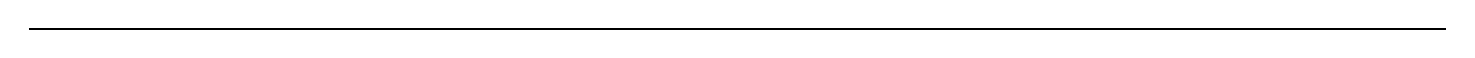
\begin{tikzpicture}
\draw[thick] (0,0) -- (18,0);
\end{tikzpicture}




\vspace{12pt}
\begin{center}
    \textbf{Report 1}
\end{center}
% \noindent \textbf{Requirements}

\vspace{12pt}

\noindent  \textbf{Team information.}

\begin{itemize}
    \item Team leader: Andruwenko Valery 
    \\Grade: 5
    \\ - Task Distribution and Coordination: As the team leader, Valery was responsible for coordinating the entire project. She assigned specific tasks to each member, ensuring that all stages of the assignment were addressed effectively. Valery also communicated with the Teaching Assistant (TA) to provide necessary information about the team and ensured that all submissions were made before the deadline. Additionally, she prepared the report about the contributions of each member, assessing their work and involvement.
    \item Team member 1: Shariev Marat 
    \\Grade : 5
    \\ - Main Coding Implementation: Marat was mainly responsible for writing the core part of the program. He worked on coding the Simplex method from scratch, ensuring that it did not rely on built-in functions, as per the assignment's requirements. His task involved implementing the algorithm for solving Linear Programming Problems (LPP), which required careful attention to the mathematical operations and logic of the Simplex method.
    \item Team member 2: Vasilev Ivan
    \\ Grade : 5
    \\- Testing: Ivan was responsible for testing the implemented program. He tested the code on different objective functions and constraints, as required by the assignment. Specifically, he ensured that the Simplex method worked across a variety of test cases, covering different numbers of variables and constraints. His role was crucial in validating the correctness and robustness of the program, and he documented any bugs or errors found during the testing phase.
    \item Team member 3: Belyaev Grigorii
    \\ Grade : 5
    \\- Research and Problem Specification: Grigorii's role involved researching tools, selecting the appropriate programming platform, and specifying the linear program to be solved. He helped identify a suitable LPP model that could be addressed by the Simplex method and ensured that the problem met all the criteria specified in the assignment. Grigorii also contributed to converting the problem into the standard form if necessary, which is an essential step in preparing the input for the Simplex algorithm.
\end{itemize}
\vspace{12pt}
\noindent     \textbf{Link to the product.}
\begin{itemize}
    \item The product is available:  
\end{itemize}

\vspace{12pt}

\noindent  \textbf{Programming language.}
\begin{itemize}
    \item Programming language:  Python
\end{itemize}

\vspace{12pt}

\noindent  \textbf{Linear programming problem.}
\begin{itemize}
\item Maximization or Minimization?
\vspace{10pt}
    \item Objective function:
    \vspace{10pt}
    \item Constraint functions:
    \vspace{5cm}
\end{itemize}



\noindent     \textbf{Input}

\vspace{12pt}
The input contains:
\begin{itemize}
    \item A vector of coefficients of objective function - $C$.
    \item A matrix of coefficients of constraint function - $A$.
    \item A vector of right-hand side numbers - $b$.
    \item The approximation accuracy $\epsilon$.
\end{itemize}

\vspace{12pt}
\noindent     \textbf{Output/Results}

The output contains:
\begin{itemize}
    \item The string "The method is not applicable!"
    
or

    \item A vector of decision variables - $X^*$.
    \item Maximum (minimum) value of the objective function.
\end{itemize}

\noindent
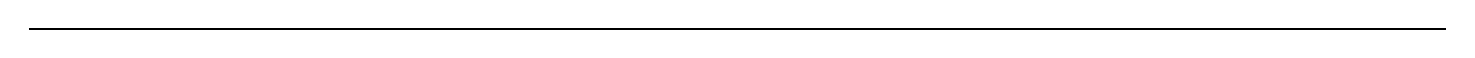
\begin{tikzpicture}
\draw[thick] (0,0) -- (18,0);
\end{tikzpicture}




\vspace{24pt}
\noindent    
\newpage
\textbf{Code}

Copy-paste your code here.

\begin{lstlisting}[language=Python, caption=Программа на Python, label=lst:python-code]
import math
c = [1,2,3]

a = [[1,1,1],
     [2,1,0],
     [0,1.5,1]]

b = [8,10,7]

epsilon = 1
class Simplex:
    
    # we define tableu:list (n:int * m:int) - matrix for simplex
    # constrains:list - to check whether tableu ratios are in the scope of them
    # var - ['x1', 'x2', 'x3', 's1', 's2', 's3']
    # basic - ['s1', 's2', 's3']
    def __init__(self, obj_function: list, constrains_matrix: list, right_hand_side_num: list, epsilon:int):
        self.constrains = constrains_matrix
        self.tableu = [[-c for c in obj_function] + [0 for i in range(len(constrains_matrix))] + [0]]
        for i in range(len(a)):
            self.tableu.append([el for el in constrains_matrix[i]] + [1 if i == j else 0 for j in range(len(constrains_matrix))] + [right_hand_side_num[i]])
        
        self.n = len(self.tableu)
        self.m = len(self.tableu[0])
        self.eps = epsilon
        self.basic = [f's{i+1}' for i in range(len(constrains_matrix))]
        self.vars = [f'x{i+1}' for i in range(len(obj_function))] + self.basic
        self.formatting = '{:'+str(self.eps + 4) + '.' + str(self.eps) + 'f}'
        self.solving = []

    # just simplex 
    def simplex_method(self):
        while True:
            enters = self.solving[0].index(min(self.solving[0]))
            if self.solving[0][enters] >= 0:
                break
            leaves = 0
            l_value = math.inf
            for i in range(1, self.n):
                if self.solving[i][enters] == 0: continue
                temp = self.solving[i][self.m-1]/self.solving[i][enters]
                if (temp < l_value):
                    leaves = i
                    l_value = temp
            if leaves == 0:
                break

            self.basic[leaves - 1] = self.vars[enters]
            
            for i in range(self.m):
                self.solving[leaves][i] /= self.solving[leaves][enters]
        
            for i in range(self.n):
                if i == leaves:
                    continue
                coef = -self.solving[i][enters] / self.solving[leaves][enters]
                for j in range(self.m):
                    self.solving[i][j] += self.solving[leaves][j] * coef

    
    def solve_maximize(self):
        self.solving = self.tableu.copy()
        self.simplex_method()
        return self.solving[0][self.m-1]
        
    
    def solve_minimize(self): 
        self.solving = self.tableu.copy()
        for i in range(self.m):
            self.solving[0][i] *= -1
        self.simplex_method()
        return -self.solving[0][self.m-1]

    
    # function to print initial tableu
    def print_initial(self):
        print("initial tableu:")
        for i in self.tableu:
            print("|", end = "")
            for j in i:
                print(self.formatting.format(j), end = " |")
            print()
        print()

    # function to print tableu after applying a Simplex method
    def print_solved(self):
        print("optimum is", self.solving[0][self.m-1])
        for i in range(len(self.basic)):
            print(self.basic[i], "=", self.solving[i+1][self.m-1])
            
        for i in self.solving:
            print("| ", end = "")
            for j in i:
                print(self.formatting.format(j), end = " |")
            print()
        print()
        lp = Simplex(c, a, b, epsilon)
        lp.print_initial()
        lp.solve_maximize()
        lp.print_solved()
\end{lstlisting}


\end{document}
